\documentclass[11pt,a4paper]{vutinfth}
\usepackage[utf8]{inputenc}
\usepackage{graphicx}
\usepackage{textcomp}
\usepackage{caption}
\usepackage{mathtools}
\usepackage{amssymb}
\usepackage[boxed,linesnumbered]{algorithm2e}
\usepackage{color}
\usepackage{subcaption}
%\usepackage[]{luatodonotes}
%\usepackage{wrapfig}



%TODO: CHANGE!
\setauthor{}{Jakob Klinger}{}{male}
\setadvisor{Ass.Prof. Dipl.-Inform. Dr.rer.nat}{Martin Nöllenburg}{}{male}%{Pretitle}{Forename Surname}{Posttitle}{male}
\setfirstassistant{Univ.Ass.}{Fabian Klute}{ M.Sc., B.Sc.}{male}
%Ass.Prof. Dipl.-Inform. Dr.rer.nat. Martin Nöllenburg
% University Assistant, M.Sc., B.Sc. Fabian Klute

\setaddress{Scherzergasse 10/8, 1020 Wien}
\setregnumber{1125755}
\setdate{25}{09}{2017}%TODO: Update

\settitle{Boundary Labeling for annotated documents}{Boundary Labeling in annotierten Dokumenten}
\setsubtitle{}{}%{TestSubtitleENG}{TestSubtitelGER}

\setthesis{bachelor}
\setcurriculum{Bachelor's programme Software \& Information Engineering}{Bachelorstudium Software \& Information Engineering} %TODO!



\newcommand{\change}[1]{\textcolor{red}{#1}}

\begin{document}

\frontmatter
%\addtitlepage{naustrian}
\addtitlepage{english}
\addstatementpage

%\begin{danksagung*}
%\todo{Ihr Text hier.}
%\end{danksagung*}

%\begin{acknowledgements*}
%\todo{Enter your text here.}
%\end{acknowledgements*}

%\begin{kurzfassung}
%\todo{Ihr Text hier.}
%\end{kurzfassung}

%\begin{abstract}
%\todo{Enter your text here.}
%\end{abstract}

\selectlanguage{english}

\tableofcontents

\mainmatter


%TODO: Abstract: \begin{abstract}...\end{abstract}

\chapter{Introduction}
Whenever additional information neets to be inserted into an existing document without altering the original text, we can make use of annotations. They usually take the form of footnotes, which require only a minimal reference in the main text, and are used for a variety of reasons - for example, to provide additional information that would hinder the text's flow if inserted directly, or as a result of a commenting tool that is used for communication between an author and their editor.
If a more obvious connection between the text and the referenced content is required, for example when lengthy comments are added, or if a change-tracking tool is used, the reference is often placed to the side of the document and visibly connected to the part of the text it is referring to. This style of annotation is easily implemented on virtual documents, since they can be hidden on demand, however if the annotations need to be included in a printed version, there are several issues that arise regarding readability of the final product and ambiguity of text-annotation assignments.

In this thesis, we will look at ways to use Boundary Labeling for this problem, which means that all annotations will be placed somewhere outside of the text they are referencing and will be visually connected to the feature they are referencing. (See also \cite{Bekos2005}) 

The guidelines on how to create suitable labelings are as follows: the connections should be as direct as possible, no important information should be obscured, and it should be easily discernable which Label belongs where. These three criteria easily come into conflict with one another, as the text usually is very dense and leaves little space for lines in between, yet one shouldn't allow them to pass through the text, as this makes the text harder to read. 

\section{Terminology and Fundamentals} %Evtl in Introduction eingliedern?
Boundary Labeling (or equivalent concepts) can be applied to a space with different geometry or more dimensions, but this thesis will only concern itself with two-dimensonal, Euclidean space.
To easily reference important concepts, some additional terminology will be introduced as well. (See Fig.~\ref{fig:term} for a visual explanation)


\begin{figure}%{r}{0.35\textwidth}
 \captionsetup{justification=centering, margin=0.75cm}
 \centering
  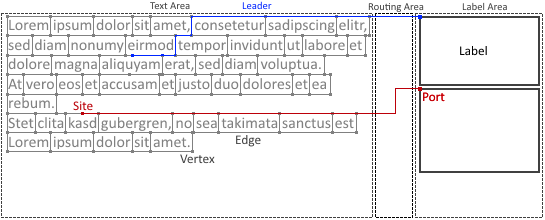
\includegraphics[scale=0.95]{GraphTerminologyExtended.png}
  \caption{Illustrated guide to the labeling terminology}
 \label{fig:term}
\end{figure}

A \emph{graph} $G=\langle V, E \rangle$ is a tuple of \emph{vertices} $V=\{v_1, v_2, ..., v_n\}$ and \emph{edges} $E=\{e_1, e_2, ..., e_m\}$. A vertex $v$ is a featureless object. %Wie  sage ich, dass die Umsetzung der Vertices sehr flexibel ist?
 Each edge $e$ is a relation between two vertices $E \subseteq V\times V$. %Edges can also be directional, or have a weight, which affects how they are treated by algorithms.
We call two vertices $u,v \in V$ \emph{adjacent}, if the edge $e=(u,v) \in E$.
 A \emph{path} $P=v_1, ..., v_h$ is an ordered sequence of vertices, where each vertex must have an edge connecting it to the subesquent one.
 \emph{Depth-first search} is a searching algorithm on a graph G that starts at a given vertex $v \in V$ and explores the graph by traversing its edges as far as possible before backtracking, and continues to do so until a pre-defined goal is met. %In our algorithm, the goal is to reach a target vertex $v_t \in V$, at which point the algorithm terminates and returns the route taken from $v_s$ to $v_t$.
% A search algorithm is \emph{monotonous} if, for each vertex $v$ and each successor $v'$ generated by the algorithm, the estimated cost of reaching the goal from $v$ is not greater than the cost of reaching $v'$ plus the estimated cost of reaching the goal from $v'$.

\emph{Polylines} are a connected series of \emph{line segments}. Line segments are straight lines that contain each point between their starting and end point. 
\emph{Labels} hold additional information and are represented as boxes containing this information. They are usually placed in the \emph{label area} which is a rectangular area designated to hold labels. It is located next to of the bigger, rectangular \emph{text area}, which contains the document's text and all \emph{sites}, the points or objects that a label's information refers to. If multiple label areas exist on different sides of the text area, we speak of \emph{multi-sided labeling}, otherwise we speak of \emph{one-sided labeling}. We will be using one-sided labeling in our implementation. Some space was left in between the text and label area, to make connecting sites to their labels easier, which we will call the \emph{routing area}. The site and the label are connected via a \emph{leader}, a polyline that can be further classified by looking at the orientation of its segments: \emph{O-Segments} run orthogonally to the border of the label area. \emph{P-Segments} run parallel to the border of the label area, and as such must be combined with other segments for the leader to reach its destination. \emph{S-Segments} are not required to have any particular orientation, and simply connect their start and ending points in a straight line.
The leader's name is created by combining the name of the segments - for example, the blue leader from Fig~\ref{fig:term} would be classified as an OPOPO-Leader.
The location where a leader connects to the label is called the \emph{port}. It can be restricted to pre-defined positions. %TODO: Re-insert monotonicity

% \textbf{Monotonous/Monotonicity:} Describes a steady progression towards a direction or goal. Will be used in this paper to indicate that there's no loss of progress made from the site to the label, effectively restricting the direction a leader can go at each bend.
%+Node für Knoten in Polylinien?

\section{Related Work}

Boundary labeling was first introduced by Bekos et al. in 2004 (see \cite{Bekos2005}), where both one-sided and multi-sided labelings with different leader types are looked into. They also showed that the optimal placement of arbitrarily-sized labels on two sides of the text area can be NP-hard by drawing comparisons to the Partition-Problem. However, a pseudo-polynomial solution exists for this problem, which was adapted to this variation of the problem.

Since then, several papers have been written about boundary labeling. One of these is \cite{Barth2015}, which looks into the readability of different leader styles. Interestingly, some leader styles perform quite well, despite the study's participants preferring others over them, with OPO-Leaders being both least preferred and the hardest to follow.

Another article using boundary labeling is \cite{Goetzelmann2006} by G{\"o}etzelmann et al., which creates boundary labeling-style annotations along other methods to label different parts of three-dimensional figures, resulting in pictures similar to what could be found in a textbook. As this algorithm works in real-time, it is suitable for labeling interactive models and allows for user interaction.


%Beispiele von suboptimalen Lösungen einfügen? (Bilder)
Boundary labeling in text documents however, is rarely discussed, and only few papers exist about this topic. The programs that employ this style of annotation often also use rather simple algorithms, to mediocre results or make extensive use of the interactivity of a digital medium, showing annotations only on demand. However, the few papers that approach this topic add interesting information to the discussion.

The paper about the Luatodonotes-Package\cite{Kindermann2014} uses several styles of drawing leaders, and came to the conclusion that leaders without bends are easier to follow, which fits with \cite{Barth2015}'s observations, which ranks OPO- and PO-Leaders lower than other variants.
However, most solutions proposed in \cite{Kindermann2014} do not consider whether a path overlaps with text or not, which results in a decrease in readability. While we do not use the routing and leader styles introduced in this paper, the results can be used in comparisons regarding readability of the main text and ease of use of the different leader styles.%Bsp-Bild einfügen!

The thesis by Loose\cite{Loose2015} on the other hand is based around only using the free space between lines and words, which produces longer leaders, and forces curves, but doesn't obscure any part of the text. The two different approaches in this paper were a clustering-based algorithm, which was previously described in \cite{Nollenburg2010}, and a flow network-based approach. Several concepts of this paper, such as the graph-based strategy and the usage of a routing area will be adopted in our thesis and it is by far the biggest influence on our approach to the problem.  %Anmerken, dass viele Konzepte hier aufgegriffen werden!

Lin et al.\cite{Lin2009} use only OPO-Leaders that have their P-Segment located outside of the text area in their paper, but allow the leaders to use the text area's border on the opposite side of the label area to route upwards or down. This allows for more labels to be placed as close as possible to their leader's source, at the cost of increasing select leaders' length and placing some labels out of order. While this is an interesting way to avoid longer leaders in general, it is hard to combine with the graph-based routing that happens inside the text area, so we won't make use of it.


\chapter{The Algorithm}
%1 Zeile Einleitung hier einfügen - zb: Kapitelübersicht
\section{Problem Specification}
We limited the leaders to use exclusively O- and P-Segments, and banned them from passing through words. We also place labels as far up as possible to maximize the space remaining for  remaining placements. Additionally, a leader isn't allowed to be any longer as is necessary to connect a given Site with its label's port.

These restrictions are implemented as follows: We divided the text $T$ into separate lines $L=\{W,H\}$ which are in turn made up of words $W$ and whitespace $H$. The remaining space between lines shall be defined as $S(l_1, l_2)$%improve on this!
with $l_1,l_2 \in L$ and will have no restrictions regarding leader placement. For each word $w \in W$, we define $R(w)$  as its bounding rectangle, which marks the space leaders aren't allowed to cross. For a graphical representation see Fig.~\ref{fig:wbound}.

\begin{figure}
 \centering
 \begin{subfigure}[b]{\textwidth}
 \centering
  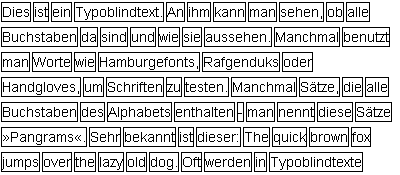
\includegraphics[]{WordBoundaries.png}
  \caption{\label{fig:wbound}}
 \end{subfigure}
 \\
 ~\\%There's probably a better way for this...
 \begin{subfigure}[b]{\textwidth}
 \centering
  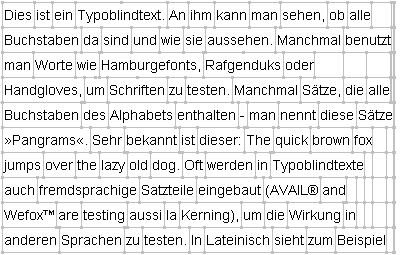
\includegraphics[]{RoutingGraph_edited.png}
  \caption{\label{fig:rgraph}}
 \end{subfigure}
 \caption{Visualization of the space reserved for the text, and the resulting graph.}
\end{figure}

Since we only allowed the Usage of O- and P-Segments in leaders, the only way for a leader to cross through a line of text is with a P-Segment through whitespace, whereas O-Segments are only usable between lines. Therefore, we can create a routing graph $G=\langle V,E\rangle$ whose Edges $E$ reflect the legal paths a leader can take within $T$.
For each whitespace character $h_x \in W$ in a given line $l_i \in L$, one vertex is placed in $S(l_{i-1},l_i)$ and $S(l_i,l_{i+1})$ each, located above or below the whitespace character, and with a maximum distance from each of its neighbouring lines. The start and end of each line also recieve a pair of vertices each. Sites will be represented by the insertion of additional vertices in $S(l_i, l_{i-1})$ on a similar height as those next to whitespace of the same line and located directly above the center point of its words $w_j$ bounding rectangle $R(w_j)$. Should either $l_{i-1}$ or $l_{i+1}$ not exist, the vertices' vertical placement will be similar to that of the previous or following line. The edges between the vertices are all perfectly horizontal or vertical, and do neither intersect with any bounding rectangle, nor any vertices other than their starting and ending vertex. The resulting graph looks similar to Fig.~\ref{fig:rgraph}.

Each edge has a capacity of 1, meaning that no more than one leader is allowed to pass through it. Leaders also aren't allowed to cross one another, as it is hard to discern between intersections and two leaders curving away from each other. This is realized by forcing leaders to incorporate as many P-Segments as early as possible while still following all previous restrictions, and forbidding leaders from entering the space to the top left of already successfully routed leader's sites.
%In our algorithm, the focus was put on keeping the text as readable as possible. This means that leaders aren't allowed to pass through words - they can only use the space between words and in between lines.
%Additionally, we wanted to maximize the usage of the label area's space, even if we have to move labels further from their sites than needed. 
%Finally, we wanted to keep the leader's length low for any given combination of labels and site placements, so every segment of a leader has to decrease the remaining distance between the site and its label's port.

%\begin{figure}
% \captionsetup{justification=centering, margin=0.75cm}
% \centering
%  \makebox[\textwidth][c]{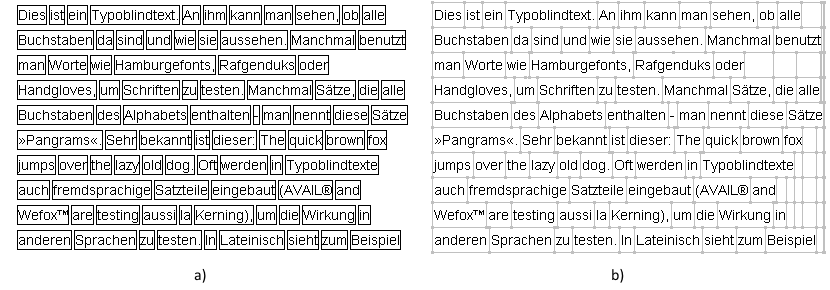
\includegraphics[scale=0.9]{FromTextToGraph.png}}
%  \caption{Visualization of the space reserved for the text, and the resulting graph.}
% \label{fig:ttg}
%\end{figure}

%These properties were modelled by creating a rectangle around each word that no leaders may pass through. If this is done for all words in a paragraph, the remaining available space for routing resembles a grid, like in Fig.\ref{fig:ttg}a.

%Since the layout encourages the usage of P- and O-segments, we decided to represent the possible routes by creating a graph which has its vertices located whenever multiple directions are available - in between lines, above or below whitespace characters. The graph's edges represent the different possible segments of a leader and connect each vertex with the closest vertices directly above, below or to the sides, given that no text is blocking the connection. The resulting graph looks similar to the one in Fig.~\ref{fig:ttg}b.

%For ease of visualisation, we limited the number of leaders per edge to one, and forbid the leaders to cross one another, as this could be mistaken for two leaders touching each other at the corners. We also decided to place the annotations in the order in which they appear in the text, and always place their port above the leader's source, which means that crossings are inevitable if a leader is located above and to the left of an earlier leader. To ensure this never happens, leaders aren't allowed to enter the top left quadrant of a source vertex, unless no routing could be found for that vertex, which means there won't be any leaders to collide with. Additionally, to keep the leader's length minimal, each leader is only allowed to move towards the source, which places a hard limit on how far up a leader is allowed to go, and restricts the possible choices at each node to edges that allow the leader to move in that direction.
%To maximize the space available to subsequent annotations, each label is placed as far up as possible. This also means that if there's no placement available that is above its leader's source, the annotation cannot be placed, as we previously restricted the leader's movement. 

%This was implemented by enclosing each word in a bounding rectangle that leaders aren't allowed to pass through.
%The leaders should also be kept as short as possible, so we restricted them to always be moving toward the label, even if the direct route is unavailable.%Wie drücke ich das als Formel aus?
%We also wanted to use the space available in the labeling area as efficiently as possible, so labels are placed as far up as possible in order to maximize the space available to future labels at the cost of increased leader length.

\section{Description}

\begin{algorithm}%{r}{0.35\textwidth}
\DontPrintSemicolon
\SetKwData{Words}{words}
\SetKwData{PrevW}{previousWord}
\SetKwData{G}{Graph}
\SetKwData{W}{w} \SetKwData{V}{v}\SetKwData{Va}{v1} \SetKwData{Vb}{v2} \SetKwData{Vc}{v3} \SetKwData{Vd}{v4}
\SetKwData{Up}{UpperVerticesList}
\SetKwData{Low}{LowerVerticesList}

\SetKwFunction{setAnn}{setAnnotation}
\SetKwFunction{NewVert}{new Vertex}
\SetKwFunction{AddVert}{addVertex}
\SetKwFunction{AddAll}{addAll}
\SetKwFunction{CEdge}{createEdgeBetween}
\SetKwFunction{PosConn}{connectBasedOnPosition}
\SetKwFunction{ClrList}{emptyList}
\SetKwFunction{getC}{getCenter}
\SetKwFunction{tLeft}{getTopLeft}
\SetKwFunction{tRight}{getTopRight}
\SetKwFunction{bLeft}{getBottomLeft}
\SetKwFunction{bRight}{getBottomRight}
\SetKwFunction{Newline}{startNewLine}

\KwData{A text with annotations,stored as a String-Array}
\KwResult{A Graph (as described above)}

 initialization\;
 
 \ForEach{\W in \Words}{
  \eIf{\W is annotation}{
   \V$\gets$\NewVert{\PrevW.\getC{}}\;
   \V.\setAnn{\W}\;
   \G.\AddVert{\V}\;
   \Up.\AddVert{\V}\;
  }{
   \If{\W is too big for the line}{
    \Newline{}\;
    \PosConn{\Up}\;
    \Up$\gets$\Low\;
    \ClrList{\Low}\;
   }
   \Va $\gets$\NewVert{\W.\tLeft{}}\;
   \Vb $\gets$\NewVert{\W.\tRight{}}\;
   \Vc $\gets$\NewVert{\W.\bLeft{}}\;
   \Vd $\gets$\NewVert{\W.\bRight{}}\;
   \;
   \G.\AddAll{\Va,\Vb,\Vc,\Vd}\;
   \Up.\AddAll{\Va,\Vb}\;
   \Low.\AddAll{\Vc,\Vd}\;
   \G.\CEdge{\Va,\Vc}\;
   \G.\CEdge{\Vb,\Vd}\;
  }
 } 
\caption{Representation of the Graph-creation algorithm in pseudocode}
\label{alg:GraphCreation}
\end{algorithm}

First, we create the graph that will be used for the routing part of the algorithm. To achieve this, we go through the annotated text word by word in reading order, and measure the length $le(w_i)$ of each word $w_i$ that is not part of an annotation to determine its placement in the text.  At this point, we can also assign a line $l_j$ to it. Afterwards, we create new vertices above and below the whitespace characters $h_k, h_{k+1}$ preceding and succeeding $w_i$. These vertices are located in the space $S(l_{j-1},l_j), S(l_j,l_{j+1})$ between the word's line and its surrounding lines $l_{j-1}$ and $l_{j+1}$, as described in the previous section. Whenever an annotation is encountered, a single vertex is added above the last non-annotation word in $S(l_{j-1},l_j)$ at $pos(h_k)+le(w_i)/2$.
For a representation of this process in pseudocode, see Alg.~\ref{alg:GraphCreation}.
%To create leaders that exclusively use the space not taken up by a word's bounding rectangle, we decided to use a graph similar to the one Loose \cite{Loose2015} used.
%As each vertex represents a physical location, they will have co-ordinates associated with them, and the vertices representing the sites will hold additional information regarding its leader and label. 
%The graph is constructed by placing vertices between the lines, located next to each corner of a word's bounding rectangle, with two consecutive words in a line sharing the two vertices associated with their adjacent corners. 
%For the sites, we inserted an additional vertex above the center of the word, which will serve as the leader's starting point. After placing all vertices, we created edges between each vertex and the closest horizontal neighbour to both sides, and between nodes that are located exactly above or below each other, and exactly one line apart. (For a representation in Pseudocode, see Alg.~\ref{alg:GraphCreation})

For the routing part of the algorithm, we work through the annotations $a \in A$ in the order they appear in the text, placing each as far up as possible, skipping any annotation that cannot be placed in a reachable position above its leader's source. We will also use fixed ports located in the top left corner of each label. %This allows us to place annotations by only knowing their port location, which can be inferred from their leader's ending point.
The routing area, which is located between the text and label areas, will be used to bridge the gap between the highest currently reachable point within the routing graph and the highest possible label placement by connecting the two via an OPO-leader.%Kann man das so sagen?

The routing algorithm itself uses only the Graph $G$ and the set of sites $V_{ann} \subset V$ which will be routed using a depth-first search algorithm, using only vertices located above or to the right of the current vertex $v_{curr}$, prioritizing moving up whenever possible. It will terminate upon reaching the right text border or if all possible paths failed to reach the text border. At this point, it will return a set with routing information for each vertex, which contains a Path $P=\{v_1, \cdots, v_n\}$, leading from the site to the text area's border, along with information on how to draw the OPO-Segment that connects to the Label's port. If the routing for any given site failed, the path consists of a single vertex - the site. (For an illustration in Pseudocode see Alg.~\ref{alg:DFS}.)

\begin{algorithm}

\DontPrintSemicolon
\KwData{A single annotation's source and its Graph}
\KwResult{A List of vertices describing the leader's path}

\SetKwData{G}{Graph}
\SetKwData{Path}{Path}
\SetKwData{Src}{Source}
\SetKwData{Curr}{currentVertex}
\SetKwData{Old}{oldVertex}
\SetKwData{Back}{backtracking}

\SetKwFunction{Top}{getTopNeighbourOf}
\SetKwFunction{Right}{getRightNeighbourOf}
\SetKwFunction{AddVert}{addVertex}
\SetKwFunction{RemVert}{RemoveVertex}
\SetKwFunction{Last}{getLastEntry}
\SetKwFunction{Below}{isBelow}
\SetKwFunction{Break}{break}

initialization\;
\While{\Curr not at right text border}{
 
 \uIf{$($\G.\Top{\Curr}$\neq null)\land \neg$\Back}{
  \Path.\AddVert{\Curr}\;
  \Curr $\gets$ \G.\Top{\Curr}\;\;
 }
 \uElseIf{\G.\Right{\Curr}$\neq null$}{
 \Path.\AddVert{\Curr}\;
  \Curr $\gets$ \G.\Top{\Curr}\;
  \Back $\gets$ False\;
 }
 \Else{
  \Back $\gets$ True\;
  \Repeat{\Curr's Position is below \Old or \Path is Empty}{
   \Old $\gets$ \Curr\;
   \Curr $\gets$ \Path.\Last{}\;
   \Path.\RemVert{\Curr}\;
  }
  \;
  \If(//No path found){\Curr not below \Old}{\Break}
 }
}
\caption{The Depth-First-Search algorithm used in the program.}
\label{alg:DFS}
\end{algorithm}

\chapter{Implementation}
The program was written in Java 1.8.0u40, using JGraphT1.0.1\cite{JGraphT} as graph library. Since we only want to create leaders that don't intersect with the text, the graph was created alongside the placement of the words on the canvas.%, as it was easy to extract measurements at this point. Due to some problems with Java's various methods of calculating linebreaks, this process was done completely by hand.
\section{Challenges}

%As the Graph's vertices represent fixed locations on the canvas, they each have coordinates associated with them, with the vertices representing the sites containing extra information, such as references to the corresponding annotation and to the leader connecting the two (if existent).
%The additional information stored in the vertices is used for both routing and drawing the leaders: The routing was done via a depth-first search algorithm that prioritized vertices located further up if possible, and vertices to the right otherwise. After the algorithm terminates, it returns  a vertex-based graph walk describing the route from the site to the border of the text area alongside information about where to draw the OPO-segment in the buffer zone if successful, or a walk containing only the starting vertex, if no valid path was found. Using this information alongside the positional data stored in the vertices, the polyline representing the leader can be drawn.


%TODO: Schönheitsfeatures, etc.
%TODO: Code genauer durchlesen und erweitern!



% For demonstration purposes, we also included another algorithm that uses S-Leaders for this section.

\chapter{Evaluation and Testing}

\section{Data generation} %\change{(Bin mit dem Titel unzufrieden, aber hier soll beschrieben werden, wie ich die einzelnen Testfälle erstellt habe.)}

\section{Testing methods}

\section{Results}

\chapter{Conclusion}

\section{Further notes}



%Section Ideas: The Program/Framework (Modellerklärung), The Algorithm(s), Implementation, Evaluation, Conclusion


\backmatter %TODO: Es gibt mehr nützliche Kommandos in VUTINFTH für zb Listen von Bildern, etc.!

\bibliographystyle{plain}
\bibliography{references}

\end{document}